% !TeX root = thesis.tex
\documentclass{master_thesis}
\addbibresource{refs.bib}

\begin{document}

\section{Research} \label{chap:research}

The research conducted for this thesis can be divided into 6 steps:

\begin{enumerate}
	\item Researching automated testing tools
	\item Pre-case study questionnaire
	\item Setting up automated testing tools in Pipedrive's component library
	\item Manual accessibility audit
	\item Comparing manual and automated testing results
	\item Post-case study questionnaire
\end{enumerate}

The first thing was to look at different automated accessibility tools that are available, test them out and see which of them would best fit the purpose of this research. The tool needed to be easy to use for everyone and not block development. The next step was to send out a questionnaire to better understand the current approaches toward accessibility among the people who work on it the most. After that, an automated accessibility tool was added to the component library and announced in relevant channels to raise awareness about it.

In parallel to observing how the tool was being used, a manual accessibility audit was conducted on the same component library. These results were then compared with the automated testing results that were obtained from testing the same version of the library with an automated accessibility tool. As the last step, a questionnaire was sent out to gather information about how the tool had been adopted.

Pipedrive has been developing a sales \ac{crm} using mostly typescript and React. Accessibility had never been a high priority and at this point, it would have not been easy to get started. Pipedrive has a design system and a React-based component library to keep the look and \ac{ux} consistent. This seemed like a good place to start solving the accessibility issues. The library is used widely in the company and developers from different teams contribute to it. For example, if a button in the reusable library gets fixed, most of the buttons in the web app that our customers use should be improved.

This should not be taken as a way to solve all accessibility problems but as a good first step. Making changes in a reusable \ac{ui} library should have a wide impact on the product's overall accessibility and without establishing a basic level of accessibility there, it would be difficult to start testing individual pages of the final product.
\flushbottom
\subsection{Research Methodology}

% \info{Methodology – The overall strategy to conduct the research, e.g. experimental, quasi-experimental, correlational, descriptive, action research, design research, ethnography – Determined by the research question - summarise the research strategy and methodology for conducting the research.}

This chapter gives an overview of the research methodologies that were used to conduct this research and explains the reasoning behind choosing them and how they were employed. It also explains the methods used for collecting and analyzing data.

\subsubsection{Literature review}

A literature review is a critical analysis of existing research and scholarly literature on a particular topic. It involves systematically reviewing, evaluating, and synthesizing existing knowledge and research findings in a specific field to identify gaps in the current knowledge and identify topics for further research \citep{Luft2022}.

As part of this research, a literature review was conducted to understand the current landscape of automated accessibility testing tools. While such tools have been available for a long time, the review aimed to determine what is already known about their strengths and weaknesses. Specifically, it sought to answer questions such as whether these tools have been tested in real-world situations and what the results were, as well as what are the main differences between them and whether some have been proven to be better than others.

EBESCO discovery service for the Academic Library of Tallinn University was used to find relevant scientific articles with the keywords "accessibility", "automated evaluation" and "continuous integration" A similar search was conducted on Google to find any nonscientific articles about the subject. The references in all of these articles were explored to identify any relevant research that should also be included.

This produced sufficiently extensive results and very soon the conclusions and references in the articles started to repeat themselves. Accessibility testing tools evolve fast and this would make older articles irrelevant to the current state of continuous accessibility testing. As a general rule, the focus was on articles that were published in the last 10 years. Older ones were only looked at when they gave more high-level overviews or methods and did not focus on comparing specific tools.

Any research papers on the subject of automated accessibility testing and any relevant articles or blog posts were looked through. Things change fast in software development and scientific publications cannot be expected to contain the most up-to-date information. That's why it was thought to be necessary to also include non-resources that have been published on reputable sites.

Many studies \citep{Alsaeedi2020, Ismailova2022, Sane2021, Vigo2013, RybinKoob2022, Duran2017} have been done to compare different accessibility testing tools using various methods. The results of these studies were reviewed and enough tools were assessed during the exploratory phase to find one that would be suitable for this case study. However, our intention was not to systematically compare them as part of this work. The comparisons that have been made by others in the past will be used as a foundation to decide which tools to use.

\subsubsection{Case study}

A case study is an in-depth analysis of a bounded system \citep{Range2023}. According to \citeauthor{Range2023}, it involves multiple forms of data collection like observations, interviews, documents, reports and analysis. The case can be a specific individual, group, community, business, organization, event or phenomenon. It can be chosen because of its uniqueness or typicality. The goal of using case study methodology is to investigate something contemporary in its real-life context.

The results of a single case study might be very subjective to that particular case and to the biased opinions of the researcher and can't always be generalized and applied to other similar situations, but the richness of detail they provide makes them fascinating and often there is a lot to learn from them \citep{Range2023}. Sometimes these insights can be applied to other similar cases. It is a good method for exploratory or critical and unusual cases.

This method was chosen to explore the possibilities of automated accessibility evaluation. An organizational case study was conducted that focused on the process of evaluating and improving the accessibility of a \ac{crm} tool called Pipedrive. In the scope of this study, an automated accessibility evaluation tool was added to Pipedrive's component library and a manual accessibility evaluation of the same library was conducted with a team of 3 designers and 1 developer working in the company.

Before implementing the new tool, a questionnaire was sent out to understand the knowledge about and approaches towards the subject of web accessibility among the company's designers and developers. At the end of the case study, another questionnaire was sent out with a focus on gaining information from people in the organization who used the tool that was added during that period. The aim was to understand if the tool was helpful, whether they had any issues using it and what was their opinion on it. The goal of both of these questionnaires was to get more detailed information about the experience of the real users of the tool.

The data collected from the automated and manual testing was organized to make it comparable. Statistical analysis was used to gain valuable insights into how well these two methods work and how they might differ from one another.

\subsection{Adding Automated Testing to Pipedrive's Component Library} \label{adding-a11y-tool}

The next step was adding an automated accessibility testing tool to Pipedrive's component library development workflow and observing its usefulness. The aim was to find a tool that can be integrated easily and that does not have a steep learning curve or add unnecessary complexity to the development workflow. Two open-source \ac{cli} tools that were mentioned in the previous research were tested to see if they would be suitable: Pa11y and Axe-core.

Pa11y CI is an accessibility test runner that is focused on \ac{ci} environments \citep{TeamPa11y2022}. It is said to work very well in \ac{ci}. The tool supports \ac{wcag} 2.0 A, AA and AAA levels and the tests can be run on multiple URLs simultaneously. Axe-core is an accessibility testing engine for websites and other HTML-based user interfaces \citep{Deque2023}. It supports \ac{wcag} 2.0 and 2.1 on levels A, AA, AAA, but needs a bit more initial setup to start testing webpages.

Storybook is used as the component explorer for Pipedrive's reusable component library's development. It is an open-source software for \ac{ui} development that allows teams to work on one component at a time \citep{storybook}. It allows rendering isolated \ac{ui} components without integrating them into the final product right away. The developers in Pipedrive use it to preview the components they are developing locally. A version of Storybook is also published on an internally available website, with all the components available for anyone in the company to see.

To run accessibility tests with either tool, the components first need to be rendered in a browser. This can be done using Storybook. Each component has stories – examples of how the component would be used in real life. The stories will be rendered in a browser inside Storybook \ac{ui}. It also has a sidebar for navigating between different examples, and controls for additional tools and documentation.
This means that to test the isolated components with pa11y CI or axe-core, Storybook's own \ac{ui} that gets rendered around the component, needs to be excluded so we can run the tests on only the actual relevant example.

Both of these accessibility testing tools are more suitable for testing whole web pages. Testing isolated components with the current setup would have required some extra steps. First, a list of all the examples for each component together with their URLs would need to be obtained in a way that it could be kept up to date every time changes are made. The next challenge would have been to isolate the components in Storybook UI to test only them and not the UI around them. This would mean building a custom solution that could be hard to maintain over time and there would have probably been more suitable solutions available already because using component libraries and Storybook is quite common.

Storybook has a wide ecosystem of add-ons and one of them is addon-a11y. It uses the same accessibility testing engine as axe-core to audit the \ac{html} of an isolated component \citep{addon-a11y}. The above-mentioned issues have already been solved here. The add-on tests only the relevant part of the \ac{html} and also provides a nice \ac{ui} inside Storybook.

As mentioned before, axe-core is an accessibility testing engine for websites and other \ac{html}-based user interfaces that supports \ac{wcag} 2.0 and 2.1 on levels A and AA \citep{Deque2023}. It has a coverage of about 20-30\% if you calculate it in a commonly used way, but they claim it to be 57\% according to their new and improved calculation method. This has been explained in more detail in the \nameref{continuous-a11y-evaluation} chapter.

Addon-a11y seemed like the best solution in this situation, so it was added to Pipedrive's component library’s Storybook. The accessibility tab is visible in every component example (Figure \ref{fig:addon-a11y}). It shows all the checks that the component has passed, all the violations that were found and any issues that could not be checked and might need manual testing. Every rule listed there also has reference to the \ac{html} node that had the violation, explanation and links to the Deque webpage with examples. This should be very useful in understanding and fixing these issues.

\begin{figure}[h]
	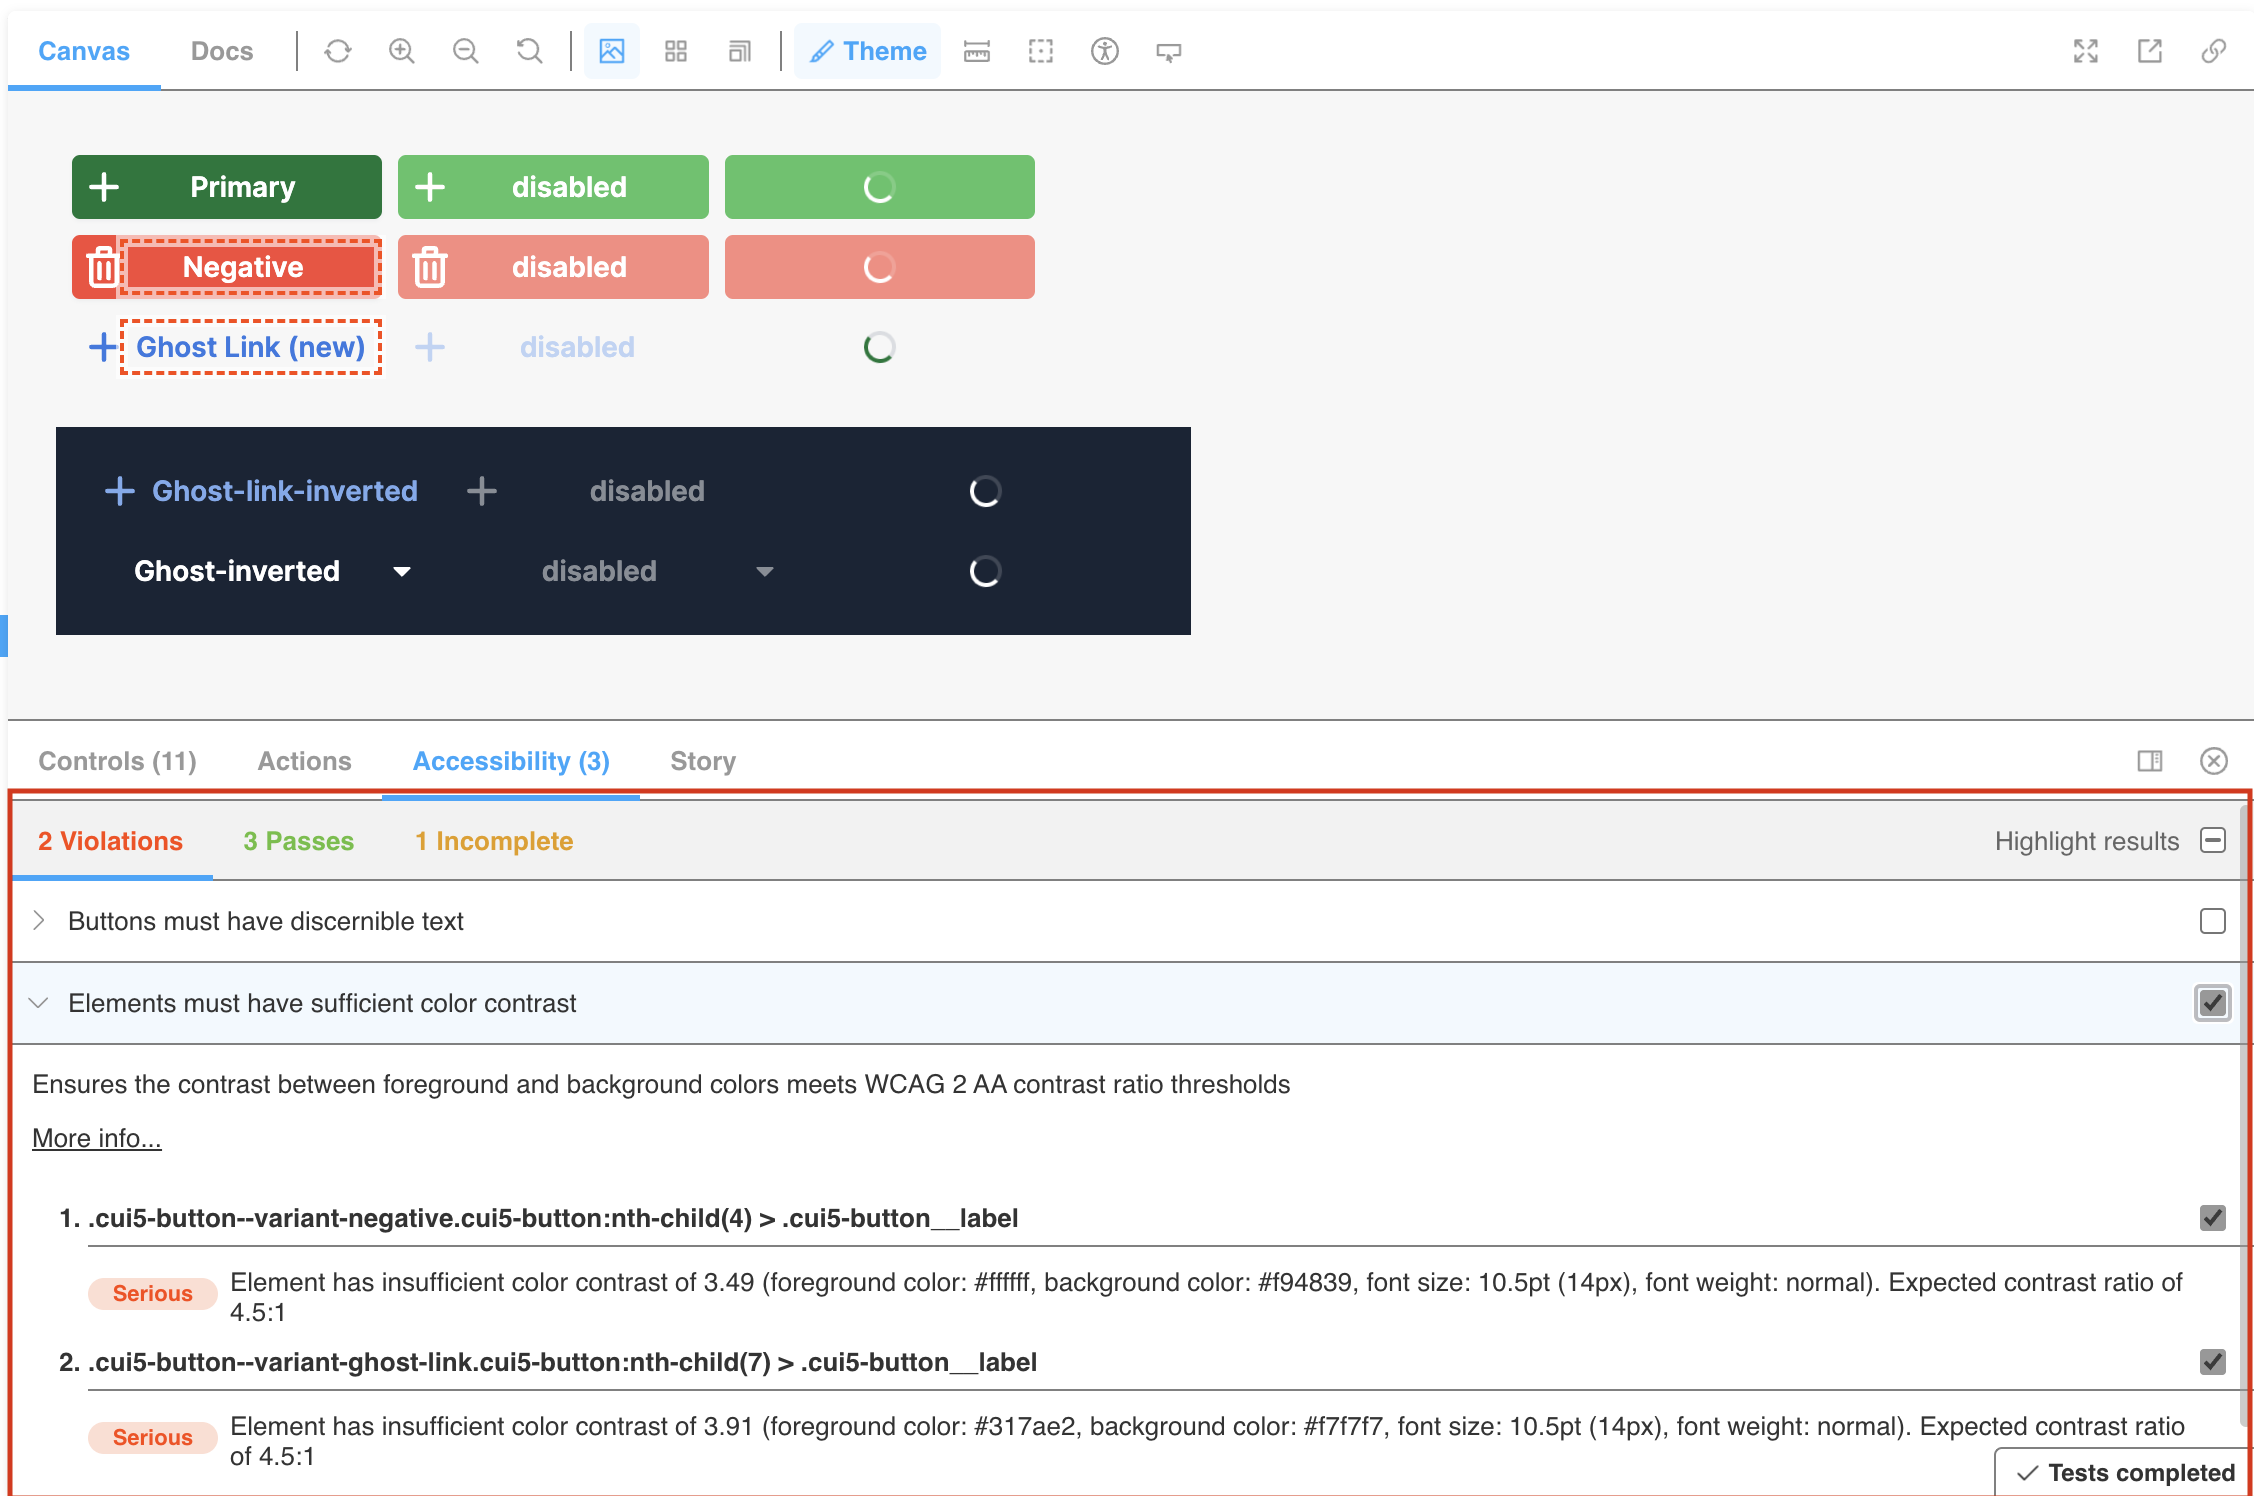
\includegraphics[width=\textwidth]{img/addon-a11y.png}
	\caption[Accessibility add-on (addon-a11y) in Storybook]{Accessibility add-on (addon-a11y) in Storybook. The accessibility panel is highlighted in yellow and the component example (story) is highlighted in green.}
	\label{fig:addon-a11y}
\end{figure}

The rules format that axe-core uses is developed by Deque Systems and is an adoption of the \ac{act} rules format developed by \ac{wai} \citep{Fiers2017}. They have a set \ac{wcag} Success Criteria that can be evaluated in a fully automated way. They are divided by \ac{wcag} guidelines version (2.0, 2.1, 2.2) and level (A \& AA, AAA) and they also have some rules for best practices in the industry that improve the user experience but might not be included in \ac{wcag} guidelines \citep{Fiers2023}.

The addon in Storybook provided a good way to test all the examples, but no way to get an overview of how many issues were found in the whole library. A summary of all the potential accessibility problems was needed to evaluate the effort and impact of making the components in this library accessible.

To get an overview of all the issues, Storybook-a11y-report \citep{Karube2020} was used to generate a report of all the violations in the whole component library. This \ac{cli} tool is meant to be used together with addon-a11y and it goes through all the examples and runs the same tests as addon-a11y to generate a summarized report. The final report links back to each component's story where the example and addon panel with all the information mentioned before can be seen (Appendix \ref{appendix:report}).

To get some data that could be compared with the results from manual testing, all the examples were examined in detail and the following data were extracted for each component (Appendix \ref{appendix:results-table}):
\begin{itemize}
	\item \textbf{unique\_violations\_detected\_for\_component} - A list of unique violations visible in the component's Accessibility tab
	\item \textbf{report\_violations} - Count of how many times the component was mentioned in the report that included all the components with all their examples. Duplicate issues can occur when the component is present in more than one example.
	\item \textbf{violations} - Count of all unique violations detected for the component. Violations that were reported in more than one example of the same component were only counted once.
	\item \textbf{true\_violations} - Count of how many of these violations are valid and relevant to this component. Violations that came from other components or elements that were included in the example just to illustrate the usage of the component were excluded.
	\item \textbf{passes\_detected\_for\_component} - A list of unique passes visible in the component's Accessibility tab
	\item \textbf{passes} - Count of all unique passes detected for the component. Passes reported in many examples were only counted once.
	\item \textbf{true\_passes} - Count of how many of these passes are valid and relevant to this component. All the passes in each component example were reviewed to decide whether they were relevant and valid. Passes that came from other components or elements that were included in the example just to illustrate the usage of the component were excluded.
	\item \textbf{explanation\_of\_false\_violations\_and\_passes} - An explanation of why each false violation and pass was not considered relevant
	\item \textbf{violations\_from\_manual\_testing\_for\_component} - A list of violations listed for each component in the manual audit report. Issues that were detected using addon-a11y, were excluded because these are listed in the automated testing report.
	\item \textbf{manual\_count} - Count of violations found in manual testing.
\end{itemize}

At the same time, a simple component library, brick-ui was set up to test anything that might not be very easy to try out in a real, actively used component library. Pipedrive's component library had more than 50 components and 414 component examples at the time of the case study. This means that any changes that affect the examples must be compatible with all examples without causing any errors. To ensure that future publishes of the library don't get blocked, any modifications made to the components or additional steps added to the development workflow must be carefully reviewed. For example, updating the component library to use the latest version of Storybook was not possible without making updates to a lot of component examples. These changes are out of the scope of this case study. Most of the concepts can be tried out with the combination of the current component library that is using Storybook 6 and brick-ui using Storybook 7.

Brick-ui was used as a quick playground to test out ideas and it provided an easy way to see if the latest version of Storybook, which was still in beta at the beginning of the case study, would have solved some of the issues that were found. Continuous improvements are being made in both  Storybook and axe-core through the maintainers and active communities around them. Brick-ui provided an opportunity to set up simple examples to illustrate some questions that came up while setting up the tools. Examples from Pipedrive's component library could not be shared, because the code is not publicly available. This made it possible to ask for help from the community and maintainers of axe-core and Storybook.

While this research was going on, development started on a new component library in Pipedrive and because the latest versions of Storybook had been explored in the simple component library, the team had the confidence to use this pre-release version of the library as the component explorer for this new library. This provided invaluable insights into an improved automated accessibility testing workflow within Storybook and an opportunity to observe the benefits of setting up automated accessibility tests from the start of the development. In this scenario, there would be no need to fix existing issues, and developers would be able to avoid them from the beginning. While this provided interesting insights, the main focus of this thesis is Pipedrive's main component library because the development of the new library is still ongoing and that makes it hard to draw any definitive conclusions.

\subsection{Manual Accessibility Audit}

The next task was conducting a manual accessibility audit of Pipedrive's main component library to get a better overview of all the issues. This approach will enable a comparative analysis of the results from manual testing and the automatically generated test report to determine the tool's strengths and weaknesses, as well as to identify any limitations when testing isolated components.

Storybook was used to render an isolated preview of each component. The accessibility add-on had already been installed, and all violations reported there were also explored. The audit team consisted of one developer and three designers. One designer considered themselves an accessibility expert. \citeauthor{Brajnik2011} cautioned that non-expert evaluators may lead to a significant drop in validity compared to expert evaluators. They suggested using at least three expert evaluators to obtain reliable results, while at least 14 evaluators may be required when the evaluators lack expertise. The audit conducted as part of this research had four evaluators, and although not all of them were experts, they all had a basic level of knowledge in the field of accessibility. Daily discussions and two longer review sessions were conducted to mitigate the lack of experience and ensure the audit's results were as reliable as possible.

Tasks were created for each component - 53 tasks in total. Everyone tested the components individually and wrote down any issues they found in a shared table. Every morning, the team had a meeting to discuss any questionable issues and to share interesting insights. Each component had 1 or more examples and the team members looked over as many of them as they thought was necessary to get an extensive overview of that specific component. The evaluators checked violations in the accessibility add-on panel, using a keyboard, and also a screen reader to navigate.

A screen reader is a software application that converts text and other on-screen information, like the layout and structure of a page, into synthesized speech, which is then delivered to the user through a speech synthesizer or refreshable braille display \citep{Watson}. It allows users to navigate and interact with web content in a non-visual way.

At the beginning of the audit, an add-on in Storybook for mocking a screen reader \citep{Lara} was used. It showed the output that a screen reader would play as audio, in text form in the add-ons panel in Storybook. Initially, it seemed like a convenient solution with rather reliable results, but further investigation revealed that the output was very different from what an actual screen reader would say.

During the rest of the audit, VoiceOver - the built-in screen reader for Apple products - was used because the our work computers are MacBooks and VoiceOver was conveniently available for us to use. There was an initial learning curve, but after that, it went quite smoothly. All the components that had already been tested with the faulty add-on, were reviewed again using VoiceOver.

The audit results were documented in a table. The barrier walkthrough method, which focused on barriers related to user interaction with the website, was used. Evaluators considered various aspects of user interactions, such as navigation, forms, and multimedia content, and looked at what issues different types of users might encounter with each component. The results were separated into 3 sections:

\begin{enumerate}
	\item Mouse user issues - using a mouse to interact with the page
	\item Keyboard user issues - using only a keyboard to do the same things
	\item Screen reader user issues - trying to do the same things and getting the same information while only using a screen reader
\end{enumerate}

This separation was seen as a good way to prioritize fixing the issues in the future. The mouse user is the user who is currently considered in all of our development and the issues they would encounter should be considered most critical. This category includes a lot of visual, color contrast, and click target size issues.

The second type of user would encounter all the issues from the first category plus everything that is unusable for them by using a keyboard. The functionalities that the user should be able to use with a mouse were explored by using only the keyboard.

The third type of user was simulated by using a screen reader. The prerequisite for this was keyboard accessibility - if it was not usable with a keyboard then it might not be usable by a screen reader. Some components actually worked better with a screen reader. Screen readers have more possibilities for navigating through elements and nested elements and this helped access some nested focusable elements that were unreachable using a keyboard.

In real life, these 3 types of users might not be so clearly separated and many issues would affect all of them, but as the intention was to come out of the audit with an actionable list, the issues needed to be prioritized in order of severity and current customer impact. These categories also mostly depend on each other, so it would make sense in most cases to start by solving mouse user issues, then keyboard user issues and then screen reader user issues.

\end{document}